\chapter{Implementacja systemu}
\section{Architektura systemu}
Aplikacja została zaprojektowana w oparciu o architekturę klient-serwer. Składa się z takich komponentów jak:
\begin{itemize}
	\item Frontend (Klient) - Interfejs użytkownika (UI), umożliwia użytkownikowi interakcje z systemem.
	\item Backend (serwer) - Warstwa logiki biznesowej, obsługuje żądania HTTP od klienta i komunikuje się z bazą.
	\item Baza danych (MongoDB) - Służy do przechowywania danych finansowych.
\end{itemize}

Komunikacja odbywa się przy pomocy protokołu HTTP/REST, a dane są w formacje JSON.
\begin{figure}[H]
	\centering
	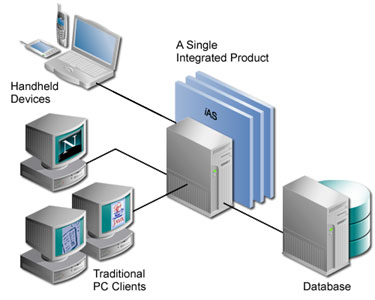
\includegraphics[width=0.7\textwidth]{images/vis.jpg}
	\caption{Tymczasowe zdjęcie architektury Klient-Serwer}
	\label{fig:KlientSerwer}
\end{figure}
\section{Backend – logika biznesowa i API}
Backend odpowiada ze przetwarzanie żądań od frontendu oraz za komunikację z bazą danych. Składa się on z kilku warstw m.in. warstwy kontrolerów, repozytoriów, czy Konfiguracji. Do komunikacji wykorzystywany jest standard REST API (ang. Representational State Transfer Application Programing Interface). Udostępnie on takie metody HTTP jak GET, POST, PUT, DELETE.
\subsection*{Jak to działa}
\begin{enumerate}
	\item Klient wysyła żądanie do określonego adresu URL (endpointu) serwera
	\item Serwer przetwarza żądanie i wykonuje operację
	\item Serwer zwraca odpowiedź w formacie JSON oraz kod stanu HTTP
\end{enumerate}
\subsection*{Opis funkcji}
Aplikacja zawiera wiele funkcji w tym Dodawanie lub usuwanie użytkowników, pobieranie listy wpłat i wypłat z konta, autoryzacja użytkowników. Wszystkie te funkcje są zawarte w odpowiednim kontrolerze. Dla każdej funkcji kontrolera został utworzony własny endpoint. Poniżej znajduje się kilka przykładów endpointów:
\begin{lstlisting}[language={Java}, caption={Przykładowe Endpointy}, label={lst:java-endpoints}]
@RestController 
@RequestMapping("/User") // Wszystkie endpointy zaczynają się od /User
	@PostMapping("/register")		// Dostęp pod POST /User/register
	@GetMapping("/search")			// Dostęp pod GET /User/search
	@PutMapping("/update/{id}")		// Dostęp pod PUT /User/update/{id}
	@DeleteMapping("/delete/{id}")	// Dostęp pod DELETE /User/delete{id}
\end{lstlisting}
Ich pełny opis znajduje się dalej w listingach (\ref{lst:java-register}, \ref{lst:java-list}, \ref{lst:java-delete}, \ref{lst:java-update})
\subsection*{Połączenie z bazą danych}
Połączenie z bazą danych odbywa się za pomocą specjalnego zasobu \textit{application.properties}, czyli właściwości aplikacji. Zawiera on wszystkie potrzebne informacje jak nazwa hosta, port na którym działa baza, nazwę bazy i ogólną konfigurację: 
\begin{lstlisting}[language={Java}, caption={application.properties}, label={lst:java-application.properties}]
spring.data.mongodb.host=${DB_HOST:localhost}
spring.data.mongodb.port=${DB_PORT:27017}
spring.data.mongodb.database=${DB_NAME:budget_management_db}
spring.data.mongodb.auto-index-creation=true
\end{lstlisting}

Mapowanie modeli na dokumenty odbywa się dzięki zależności Spring Data MongoDB. Utworzenie klasy na przykład konta wymaga podania @Document przed klasą. Dzięki temu model będzie mógł być konwertowany do formatu dokumentu.
\begin{lstlisting}[language={Java}, caption={Fragment modelu Account}, label={lst:java-Account}]
@Document
public class Account {
	@Id
	private String id;
	private String name;
	@Size(min = 25, max = 25)
	@Indexed(unique = true)
	private String number;
	private Currency currency;
	private String userId;
	...
\end{lstlisting}
\subsection*{Konfiguracja i bezpieczeństwo}
Opcje konfiguracji i bezpieczeństwa to bardzo ważna część aplikacji. Odpowiada za sposób generowania tokenów, które następnie zostaną wykorzystane do tworzenia ciasteczek. Odpowiada też za walidację oraz dostęp do metod. Określa jakie funkcje dostępne są dla użytkowników nieautoryzowanych, a które mogą zostać wywołane przez tych posiadających autoryzację. 
\subsection*{Przykładowe fragmenty kodu}
\subsubsection*{rejestracja}
\begin{lstlisting}[language={Java}, caption={Rejestracja użytkownika}, label={lst:java-register}]
/**
* Rejestracja użytkownika.
* @param user Obiekt użytkownika zawierający dane do rejestracji w formacie JSON.
*             Wymagane pola: login, password, role.
*/
@PostMapping("/register")
public String register(@Valid @RequestBody User user) {
	user.setPassword(passwordEncoder.encode(user.getPassword()));
	userRepository.insert(user);
	return "Rejestracja udana";
}
\end{lstlisting}
\subsubsection*{Lista użytkowników}
\begin{lstlisting}[language={Java}, caption={Lista użytkowników}, label={lst:java-list}]
@GetMapping("/list")
public Iterable<User> getUser() {
	return userRepository.findAll();
}
\end{lstlisting}
\subsubsection*{Usuwanie użytkownika}
\begin{lstlisting}[language={Java}, caption={Usuwanie użytkownika}, label={lst:java-delete}]
@DeleteMapping("/delete/{id}")
public void deleteUser(@PathVariable String id) {
	userRepository.deleteById(id);
}
\end{lstlisting}
\subsubsection*{Edycja użytkownika}
\begin{lstlisting}[language={Java}, caption={Edycja użytkownika}, label={lst:java-update}]
@PutMapping("/update/{id}")
public void updateUser(@PathVariable String id, @RequestParam String login) {
	User user = userRepository.findById(id).orElseThrow(() -> new RuntimeException("User not found"));
	user.setLogin(login);
	userRepository.save(user);
}
\end{lstlisting}
\subsection*{Testy jednostkowe}
Aplikacja posiada również możliwość testowania poprawności działania metod. Testowanie polega na sprawdzeniu, czy funkcja zwraca odpowiednią odpowiedź z serwera, na przykład w przypadku nieautoryzowanego dostępu do funkcji w odpowiedzi od serwera powinniśmy otrzymać błąd 401 (Unauthorized). W przypadku, gdy wszystko zakończy się powodzeniem otrzymamy sygnał 200 (OK). Kody błędów znajdują się w tabeli (Nie ma jeszcze). Do testowania aplikacji wykorzystuje bibliotekę JUnit w wersji 5.
\begin{lstlisting}[language={Java}, caption={Przykładowy test}, label={lst:java-UnitTest}]
@Test
public void createTransferHandlesNegativeTransferAmount() throws Exception {
	this.mockMvc.perform(MockMvcRequestBuilders.post("/Transaction/create/transfer")
	.contentType("application/json")
	.content("{\"fromAccountNumber\":\"1234567890122234569012335\",\"toAccountNumber\":\"1234567890122234569012335\",\"amount\":-50.0}"))
	.andExpect(status().is4xxClientError())
	.andExpect(content().string("amount: must be greater than 0"));
}
\end{lstlisting}
\section{Frontend – interfejs użytkownika}
Warstwa prezentacji systemu, czyli to z czym użytkownik wchodzi w interakcje nazywamy frontendem. Została zrealizowana przy pomocy biblioteki React oraz narzędzia Vite. Kod źródłowy programu został napisany w TypeScipt. Komunikacja została zapewniona dzięki protokołowi HTTP/REST. Powoduje to niezależność frontendu od backendu.
\subsection*{Struktura projektu}
Projekt jest podzielony na moduły:
\begin{itemize}
	\item Assets - przechowywanie statycznych elementów strony (np. ikony),
	\item Models - Zawiera typy utworzone na potrzeby działania funkcji,
	\item Services - Odpowiada za komunikacje z backendem,
	\item Styles - Przechowuje style w formacie .css,
	\item Context - Obsługuje globalny stan aplikacji,
	\item Components - Zawiera widoki stron i wszystkie elementy takie jak formularze
\end{itemize}
\subsection*{Komunikacja z API}
Komunikacja z backendem odbywa się dzięki bibliotece axios, która odwołuje się do endpointów strony. Poniżej znajduje się przykładowa funkcja wyszukująca konta.
\begin{lstlisting}[caption={Funkcja wyszukująca wszystkie konta użytkownika}, label={lst:TS-service1}]
export const fetchAccounts= async (): Promise<Accounts[]> =>{
	const id = await fetchUserId();
	try {
		const response = await axios.get(`http://localhost:8080/Account/get/${id.id}`, {
			withCredentials: true,
			headers: {
				'Content-Type': 'application/json'
			}
		});
		return await response.data;
	} catch (error: any) {
	throw new Error(error.message || "Wystąpił błąd podczas pobierania kont");
	}
}
\end{lstlisting}

\subsection*{UI}
Interfejs użytkownika jest przejrzysty i łatwy w obsłudze. Wiele elementów na stronie zostało wykorzystane z biblioteki Ant Design, która jest jedną z popularniejszych bibliotek dla React'a. Pozwala ona na tworzenie formularzy, wykresów liniowych, przycisków, ikon i wielu innych przydatnych elementów strony. Użytkownik może personalizować motyw strony (jasny/ciemny), sprawdzić szczegóły profilu lub przejrzeć historię i dane swoich kont bankowych, które ma przypisane do konta.
\subsection*{Stan aplikacji i interakcje}
Stany są jednym z kluczowych funkcji, które wykorzystuje się w aplikacjach opartych o React. Wykorzystują funkcję haków (hook), które pozwalają używać stanów bez konieczności posiadania klasy. Do zarządzania stanami możemy użyć funkcji useState lub useEffect. Funkcja useState pozwala nam ustawić jakiś status podczas działania strony. Prostym przykładem będzie zmiana motywu strony przez użytkownika. Wtedy status zmienia się z light na dark. UseEffect pozwala wykonać jakąś funkcję lub działanie i wpłynąć na to jaki status zostanie ustawiony. Poniżej znajdują się przykłady zastosowań dla obu funkcji.
\begin{lstlisting}[caption={Wykorzystanie stanów}, label={lst:TS-states}]
const [loginData, setLogin] = useState<string | null>(null);
	
useEffect(() => {
	const fetchLoginData = async () => {
		try {
			const users = await fetchUsers();
			setLogin(users.join('\n'));
		} catch (err: any) {
			message.error(err.response?.data?.error || err.message);
		}
	};
	fetchLoginData();
}, []);
\end{lstlisting}
\section{Przepływ danych}
Aplikacja przechowuje dane w postaci dokumentów bazy NoSql MongoDB. Backend komunikuje się z bazą poprzez warstwę repozytoriów i pobiera z niej informacje w formacie JSON, następnie odpowiednio sformatowane dane przesyła odpowiednim endpointem do frontendu, gdy zostanie wywołana odpowiednia metoda.
\subsubsection*{Przykładowy przepływ danych}
Poniżej znajduje się sposób przepływu danych dla funkcji logowania aplikacji:
\begin{enumerate}
	\item Użytkownik odpala formularz na stronie i wprowadza dane.
	\item Frontend wysyła żądanie HTTP do backendu.
	\item Backend przetwarza dane i porównuje je z tymi znajdującymi się w bazie.
	\item Wynik zwraca w formacie JSON.
	\item Frontend aktualizuje widok użytkownika.
\end{enumerate}
\begin{lstlisting}[caption={Przykład przesyłanych danych między frontendem, a backendem}, label={lst:TS-service1}]
[{
	"fromAccountNumber": "3620457673958599558548379",
	"toAccountNumber": "1234567890122234561012335",
	"amount": 50.0,
	"description": "test",
	"transactionId": "68dfb1d240d00a2221f78809"
},
{
	"fromAccountNumber": "3620457673958599558548379",
	"toAccountNumber": "1234567890122234561012335",
	"amount": 150.0,
	"description": "test",
	"transactionId": "68dfb1d740d00a2221f7880b"
}]
\end{lstlisting}
\section{Integracja komponentów}
Komponenty są uruchamiane w oddzielnych kontenerach Dockera. Plik compose.yml pozwala jednocześnie uruchomić bazę danych, backend i frontend przy pomocy jednego polecenia: \textit{docker compose up}.
\begin{lstlisting}[caption={Budowanie obrazu - Dockerfile}, label={lst:Docker-build}]
FROM maven:3.9.10-eclipse-temurin-21
WORKDIR /app
COPY pom.xml .
COPY src ./src
EXPOSE 8080
CMD ["mvn", "spring-boot:run"]
\end{lstlisting}
\section{Przykładowe fragmenty kodu i funkcje}
Wywalić przykłady z wcześniej i wrzucić je tutaj? Czy tutaj umieścić coś jeszcze? wszystkie przykłady dałem wcześniej.